\SECTION{Evaluation}\label{sec:evaluation}
In this section, we evaluate the runtime overhead and real-time
performance of Linux-RTXG.
The runtime overhead is classified into interrupt interception,
independent synchronization, and priority-driven scheduling in Linux.
We demonstrate that the overhead of our LKM-based real-time scheduler
for GPU applications is acceptable.
The real-time performance is verified in terms of QoS management and
prioritization using both synthetic workload and real-world
applications on top of three different device drivers -- NVIDIA,
Nouveau, and Gdev.
We demonstrate that multiple GPU applications co-scheduled by our
LKM-based real-time scheduler are successfully prioritized and
maintained at the desired frame rate even in the presence of high CPU
load.

Experiments are limited to GPU scheduling performance given that CPU
scheduling performance has already been demonstrated in previous
work~\cite{kato2009loadable}.
Considering the results of this work and those from the previous work,
it is clarified that both emerging GPU applications and traditional CPU
applications can be scheduled according to priorities and resource
reserves using LKMs, without modifying the Linux kernel and device
drivers.

\SUBSECTION{Experimental Setup}
Our experiments were conducted using the Linux kernel 3.16.0, an NVIDIA
Geforce GTX680 GPU, a 3.40 GHz Intel Core i7 2600 (eight cores including
two hyperthreadling cores), and 8 GB main memory.  
GPU application programs were written in CUDA and compiled by NVCC v6.0.1.
We used the NVIDIA 331.62 driver and Nouveau Linux-3.16.0 driver with
NVIDIA CUDA 6.0 and Gdev. 

\SUBSECTION{Interrupt Interception Overhead}
We measured the interrupt interception overhead using the Nouveau GPU
driver to quantify the overhead of interception in varied interrupt
types. 
As performance metrics, we adopted elapsed time from the beginning to
the end of the ISR.

\begin{figure*}[!t]
\begin{minipage}[t]{0.33\hsize}
\begin{center}
\raisebox{-3mm}{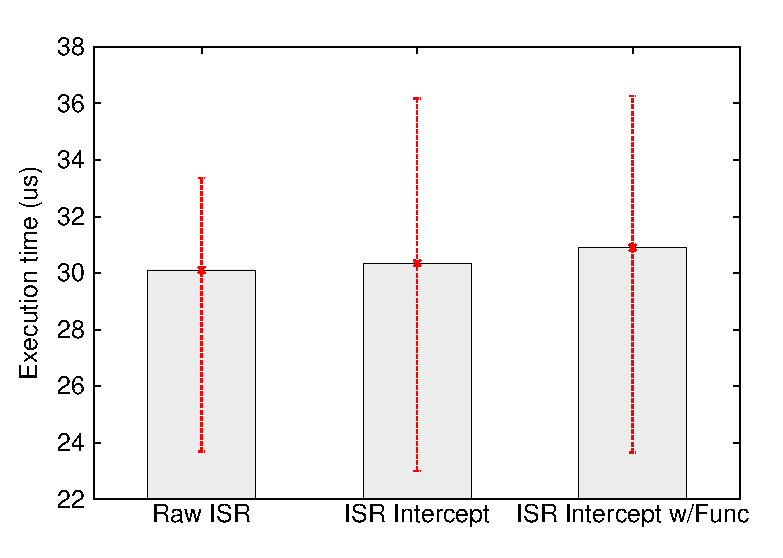
\includegraphics[width=62mm]{img/interrupt}}
\end{center}
\caption{\small{Interrupt interception overhead. \newline \,}}
\label{fig:irq_overhead}
\end{minipage}
\begin{minipage}[t]{0.33\hsize}
\begin{center}
\raisebox{-1mm}{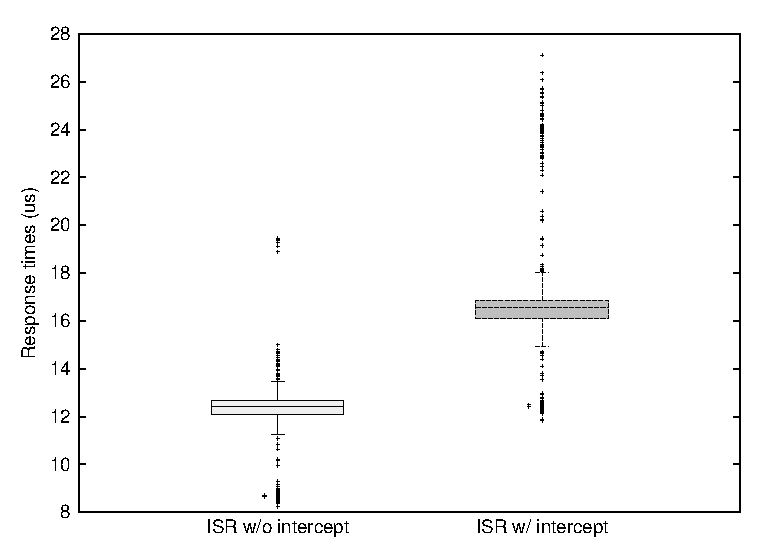
\includegraphics[width=62mm]{img/interrupt_response}}
\end{center}
\caption{\small{Impact of interrupt interception.}}
\label{fig:response}
\end{minipage}
\begin{minipage}[t]{0.33\hsize}
\begin{center}
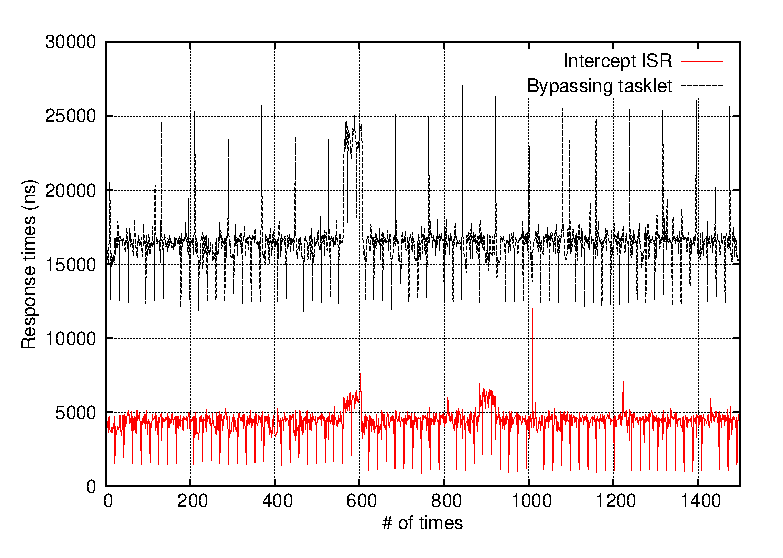
\includegraphics[width=62mm]{img/tasklet_vs_interrupt}
\end{center}
\caption{\small{Comparison of ISR and tasklet.}}
\label{fig:bottomvstasklet}
\end{minipage}
\end{figure*}

Figure~\ref{fig:irq_overhead} shows the overhead of interrupt interception.
``Raw ISR'' represents the original implementation of ISR.
``ISR Intercept'' represents the modified ISR with the interrupt
interception mechanism, while ``ISR Intercept w/Func'' includes the
overhead of identifying the ISR and calling the scheduler thread in
addition to ``ISR Intercept''.
The average execution time in 1000 executions is presented with error
bars.

Comparing Raw ISR and ISR Intercept, the overhead of introducing the
interrupt interception mechanism was $247ns$, which is only $0.8\%$ of
Raw ISR.
Similarly, the overhead for ISR Intercept w/Func was $790ns$, which is
only $2.6\%$ of Raw ISR.
This result indicates that the interrupt interception overhead is not
significant at all for total performance.

We next compare response times of ISR with and without interrupt
interception, as shown in Figure~\ref{fig:response}.
The response time is defined by the elapsed time from the beginning of
interrupt processing to the point where the interrupt type (e.g., timer,
compute, FIFO, and GPIO) is identified. 
According to the result, the impact of interrupt interception brings
1.4x longer response times.

We also compared response times when interrupt interception is
self-contained in the ISR (top-half) and when it is expanded to the
tasklet (bottom-half).
This comparison differentiates Linux-RTXG from GPUSync in performance,
since GPUSync intercepts the $tasklet\_schedule()$ on top of the
proprietary driver, while Linux-RTXG realized ISR-based interception.
In this case, the start time of measuring the response time is set at
the function call to $do\_IRQ$.
Figure~\ref{fig:bottomvstasklet} shows the result of this comparison.
As can be seen, the tasklet-based approach requires about 5x longer
response times than the IRQ-based approach.
This occurs because the tasklet is typically called after significant
ISR processings.

\SUBSECTION{Independent Synchronization Overhead}
We next quantify the overhead of the independent synchronization
mechanism.
This mechanism must call $rtx\_gpu\_notify()$ at the time of requested
synchronization (e.g., after launching a GPU kernel).
To use this mechanism, some initialization procesure is also required.
In this measurement, the overhead is defined by the execution time of
corresponding APIs.

\begin{figure}[!t]
\begin{center}
\subfigure[Overhead of initialization]{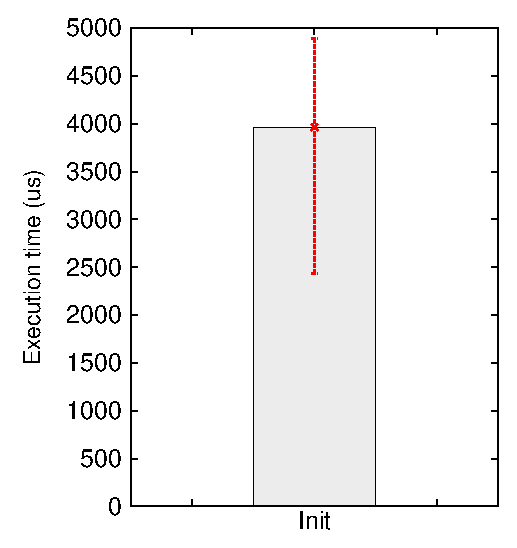
\includegraphics[width=0.23\textwidth]{img/irq_rise_init.eps}}\subfigure[Overhead of notification]{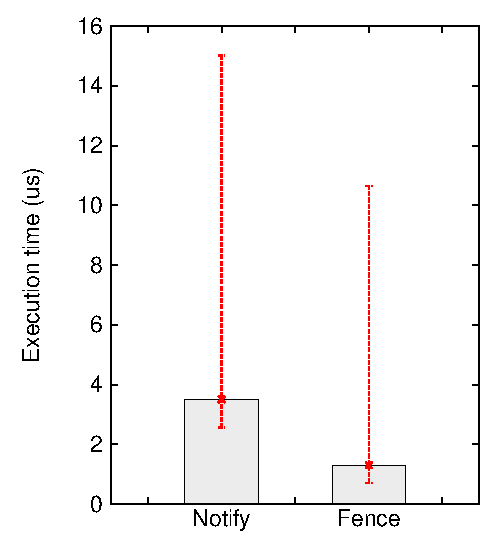
\includegraphics[width=0.22\textwidth]{img/irq_rise_notify.eps}}
\caption{Independent synchronization overhead.}
\label{fig:irq_rise_overhead}
\end{center}
\end{figure}

Figure~\ref{fig:irq_rise_overhead} shows that the initialization
overhead could reach 5000$us$, whereas the notification overhead is no
more than a few microseconds.
The initilization procedure calls a Linux process to allocate indirect
buffers and control registers for several GPU engines.
Albeit a significant overhead, the application program is not much
affected by this procedure, since it is called only once at the
beginning.
On the other hand, the notification overhead is not a major
consideration for the application program, though it is a little
scattered due to an ioctl system call.
When NOTIFY is used to set notificaiton, the overhead was $3.5us$, while
it was reduced to $2us$ when FENCE is used.

\SUBSECTION{Scheduling Overhead}\label{sec:eval:sched_overhead}

\begin{figure}[!t]
\begin{center}
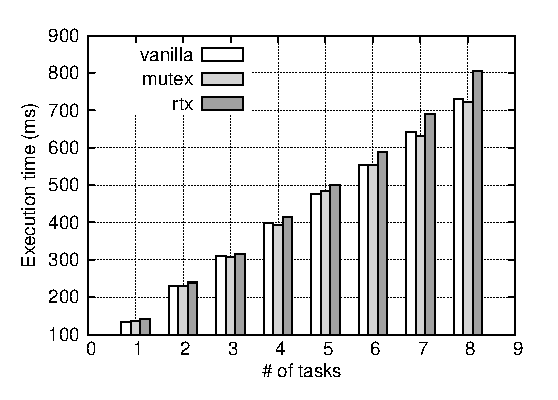
\includegraphics[width=.44\textwidth]{img/sum_task.eps}
\caption{Scheduling overhead.}
\label{fig:fp_task_overhead}
\end{center}
\end{figure}

We now evaluate the scheduling overhead posed by the presented
Linux-RTXG scheduler.
We executed three synthetic tasks -- (i) vanilla, (ii) mutex, and (iii)
rtx -- to measure the overhead. 
These tasks are based on the microbenchmark program provided by the Gdev
project, which tests a GPU loop function.
%details
We modified this program to generate multiple GPU tasks by the $fork()$
system call.
Each task releases a job ten times periodically, each of which includes
the data transfer between the CPU and the GPU, followed by GPU kernel
execution.
The rtx task was scheduled by Linux-RTXG.
The mutex task was limited to a single GPU kernel by using explicit
mutual exclusion control similar to the rtx task.
The vanilla task was not changed from the original microbenchmark
program.
The CPU scheduling policy was set to $SCHED\_FIFO$, while the GPU
scheduling policy is also based on fixed priorities with GPU resource
reservation, called the BAND scheduling policy~\cite{kato:gdev}.
The independent synchronization mechanism is employed with NOTIFY.

We measured the average time in 100 times of GPU task execution (1000 jobs).
The result is provided in Figure~\ref{fig:fp_task_overhead}.
The scheduling overhead increases in proportion as the number of tasks,
because the time consumed in queueing GPU tasks is increased. 
The maximum overhead correponds to $10\%$ of the vanilla task at eight
tasks.

\SUBSECTION{Prioritization and QoS Performance}
Experiments were also performed to evaluate prioritization and QoS
performance for GPU applications provided by Linux-RTXG.
We evaluated these pieces of performance of Linux-RTXG on both the
proprietary driver (NVIDIA) and the open-source driver (Nouveau), as
compared to the built-in kernel approach (Gdev).

\begin{figure*}[!t]
\begin{minipage}[t]{0.33\hsize}
\begin{center}
\subfigure[{\small FIFO on NVIDIA}]{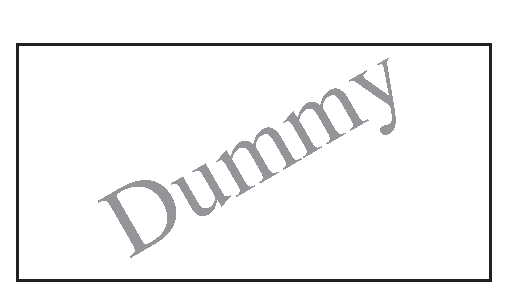
\includegraphics[width=62mm]{img/fifo_rtx_nvidia}} 
\label{fig:fifo_rtx_nvidia} \\
\subfigure[{\small BAND on NVIDIA}]{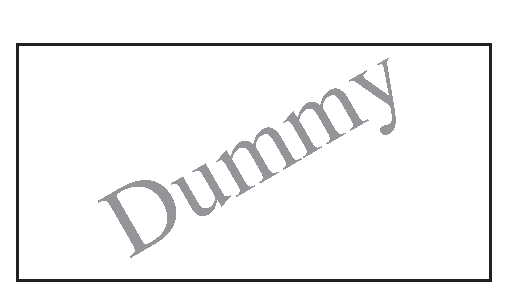
\includegraphics[width=62mm]{img/band_rtx_nvidia}}
\label{fig:band_rtx_nvidia}
\label{fig:rtx_nvidia}
\end{center}
\end{minipage}
\begin{minipage}[t]{0.33\hsize}
\begin{center}
\subfigure[{\small FIFO on Nouveau}]{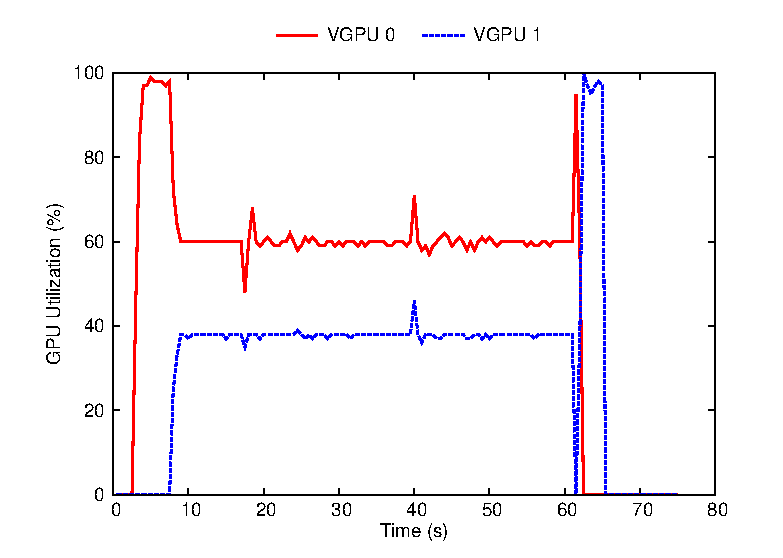
\includegraphics[width=62mm]{img/fifo_rtx}}
\label{fig:fifo_rtx} \\
\subfigure[{\small BAND on Nouveau}]{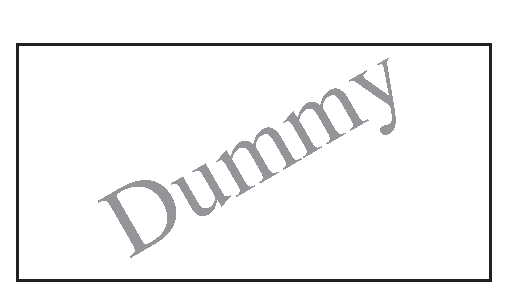
\includegraphics[width=62mm]{img/band_rtx}}
\label{fig:band_rtx}
\label{fig:rtx_nouveau}
\end{center}
\end{minipage}
\begin{minipage}[t]{0.33\hsize}
\begin{center}
\subfigure[{\small FIFO on Gdev}]{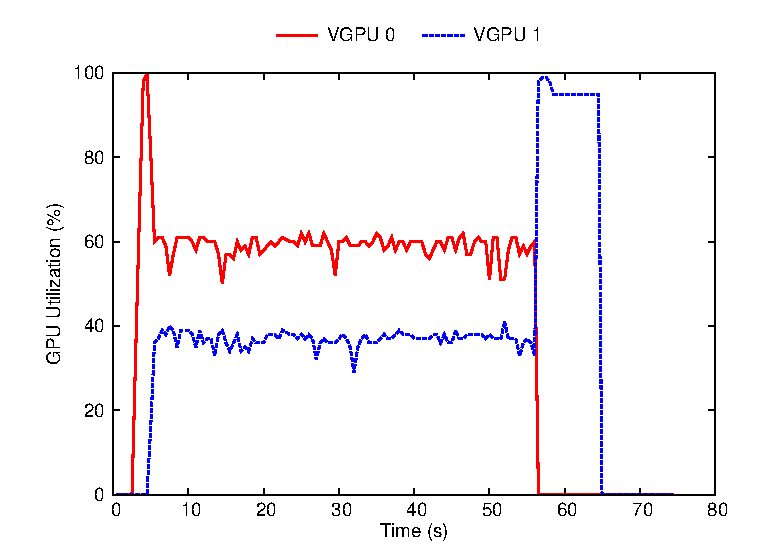
\includegraphics[width=62mm]{img/fifo_gdev}}
\label{fig:fifo_gdev} \\
\subfigure[{\small BAND on Gdev}]{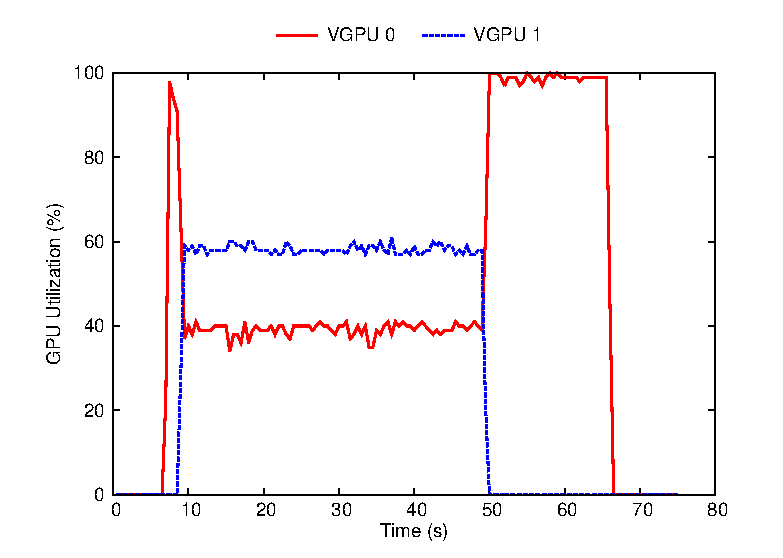
\includegraphics[width=62mm]{img/band_gdev}}
\label{fig:band_gdev}
\label{fig:gdev_usage}
\end{center}
\end{minipage}
\caption{GPU utilization of two tasks. Each task executes different
types of GPU-intensive workloads with specified GPU reserves (VGPU0 =
 40\%, VGPU1 = 60\%).}
\label{fig:utilize}
\end{figure*}

\begin{figure}[!t]
\begin{center}
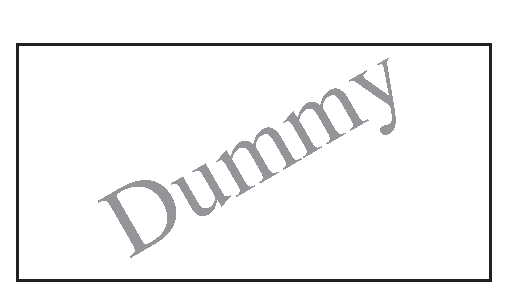
\includegraphics[width=0.4\textwidth]{img/band_rtx_fair}
\caption{Utilization of four tasks with the Linux-RTXG's BAND VGPU scheduling. Each tasks had a equal workload and a equal GPU resource allocation.}
\label{fig:band_rtx_fair}
\end{center}
\end{figure}

QoS management indicates if GPU time of the corresponding task is
guaranteed.
We evaluated QoS performance by observing how well the tasks are
isolated.
First, we measured GPU utilization when running two GPU tasks.
Each GPU task has a unique workload with a different size of GPU
reserve.
One task was allocated to VGPU0, and given $40\%$ of GPU reserve.
This task with a high priority has $1.2$ times higher workload than the
other, which was allocated to VGPU1 with $60\%$ of GPU reserve.
The VGPU1 task was scheduled to start approximately $5s$ after the VGPU0
task.

Figure~\ref{fig:utilize} (a) shows the result obtained under the FIFO
scheduling policy on the NVIDIA Driver, while that under the BAND
scheduling policy is shown in Figure~\ref{fig:utilize}(b).
The corresponding results on the Nouveau GPU driver are shown in
Figures~\ref{fig:utilize} (c) and (d).

Since VGPU0 has higher workload than VGPU1, the GPU tasks are performed
in accordance with their workload as shown in Figures~\ref{fig:utilize}
(a) and (c).
On the other hand, the GPU resource reservation mechanism provided by
Linux-RTXG can successfully perform the GPU tasks in accordance with
their reserves as indicated in Figures~\ref{fig:utilize} (b) and (d).
It is important to remind that these prioritization and resource
reservation for GPU applications can be achieved without modifying the
OS kernel and device drivers in Linux-RTXG.

The maximum error of the VGPU1 task was approximately $3\%$ under the
BAND scheduling policy on the NVIDIA driver, while that of the VGPU0
task was approximately $5\%$.
Using the Nouveau driver, those numbers were $2\%$ and $6\%$,
respectively.
The large spikes occurred due to GPU kernel overruns.

In addition to our loadable kernel approach, we compared performance
with the prior work, Gdev.
The Gdev scheduling results are shown in Figures~\ref{fig:utilize} (e)
and (f).
Almost no performance loss is imposed on Linux-RTXG as compared to
Gdev.
In detail, using the Gdev scheduler, the maximum error of the VGPU1 task
was approximately $3\%$ under the BAND scheduling policy, while that of
the VGPU0 task was $5\%$.
There is also a large variation on a time basis when using the Gdev
scheduler.
This is because the runtime functions of Gdev must be called in the
kernel space, where other system calls can easily block their operation.

We next measured GPU utilization running four GPU tasks.
Each GPU task has the same workload and the same GPU reserve on a
different VGPU.
Figure~\ref{fig:band_rtx_fair} shows the isolation result of this
scenario.
The maximum error of VGPUs was at most appropriately 9\%, which is
incurred due to the timing of budget replenishment and synchronization
latency.
In fact, this result almost matches the previous work from
Gdev~\cite{kato:gdev} using the built-in kernel approach.
As a result, the independent synchronization mechanism employed in
Linux-RTXG does not sacrifice scheduling performance.

\begin{figure*}[!t]
\begin{minipage}[t]{0.33\hsize}
\begin{center}
\subfigure[{\small NULL.}]{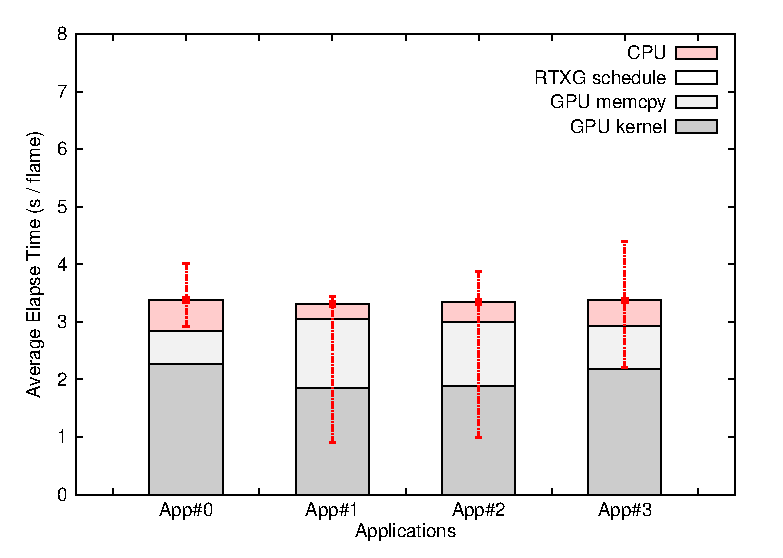
\includegraphics[width=62mm]{img/real_null_null_withoutload}}
\label{fig:real-null_null}
\subfigure[{\small FP.}]{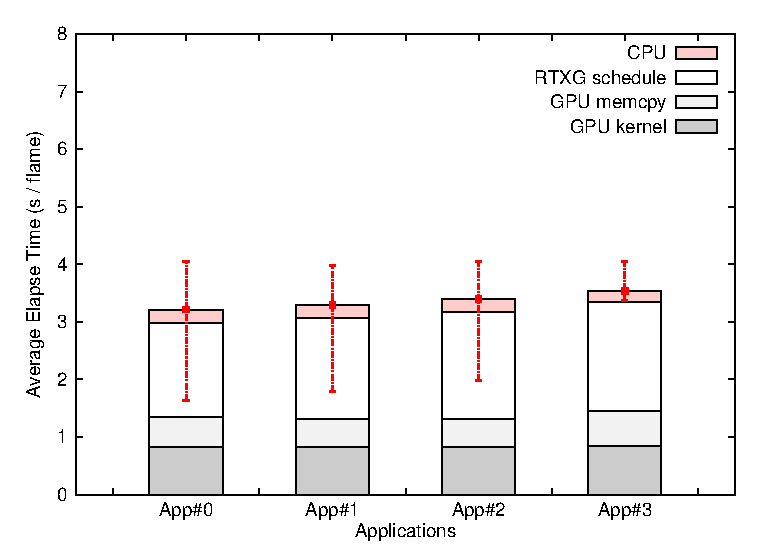
\includegraphics[width=62mm]{img/real_prio_null_withoutload}}
\label{fig:real-prio_null}
\end{center}
\end{minipage}
\begin{minipage}[t]{0.33\hsize}
\begin{center}
\subfigure[{\small BAND.}]{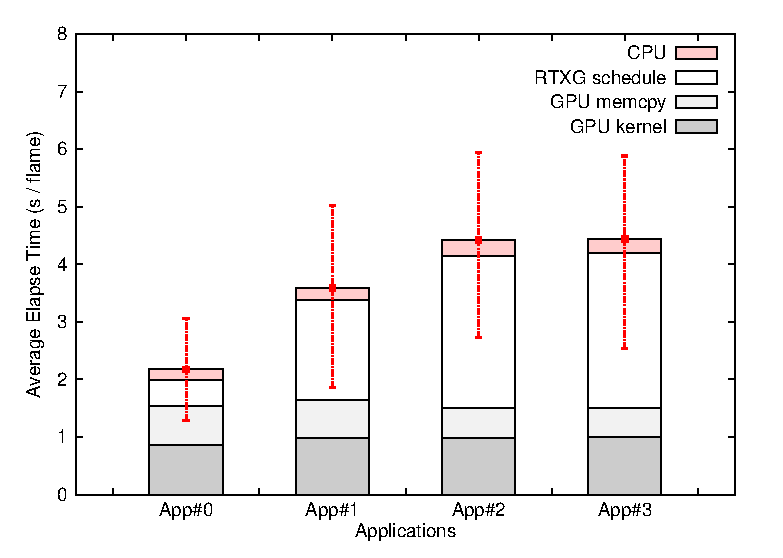
\includegraphics[width=62mm]{img/real_prio_band_withoutload}}
\label{fig:real-prio_band}
\subfigure[{\small BAND with high CPU load.}]{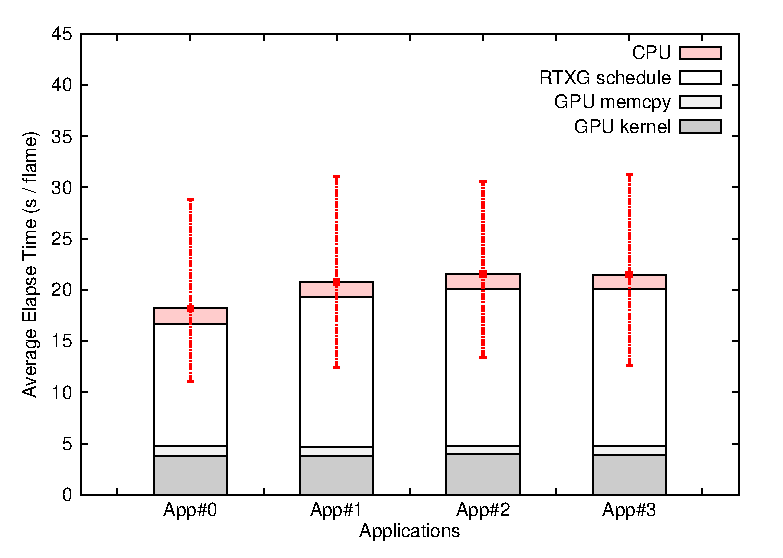
\includegraphics[width=62mm]{img/real_prio_band_withhighload}}
\label{fig:real-prio_band-hiload}
\end{center}
\end{minipage}
\begin{minipage}[t]{0.33\hsize}
\begin{center}
\subfigure[{\small NULL with high CPU load.}]{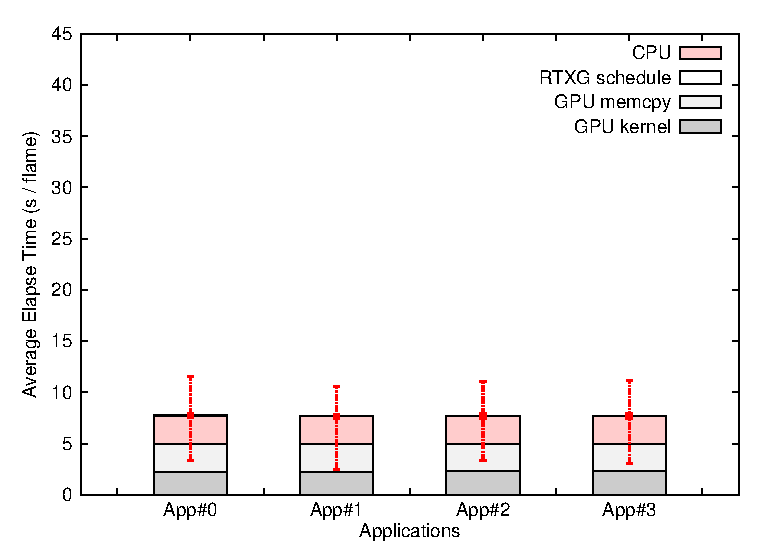
\includegraphics[width=62mm]{img/real_null_null_withhiload}}
\label{fig:real-null_null-hiload}
\subfigure[{\small FP and BAND with high CPU load.}]{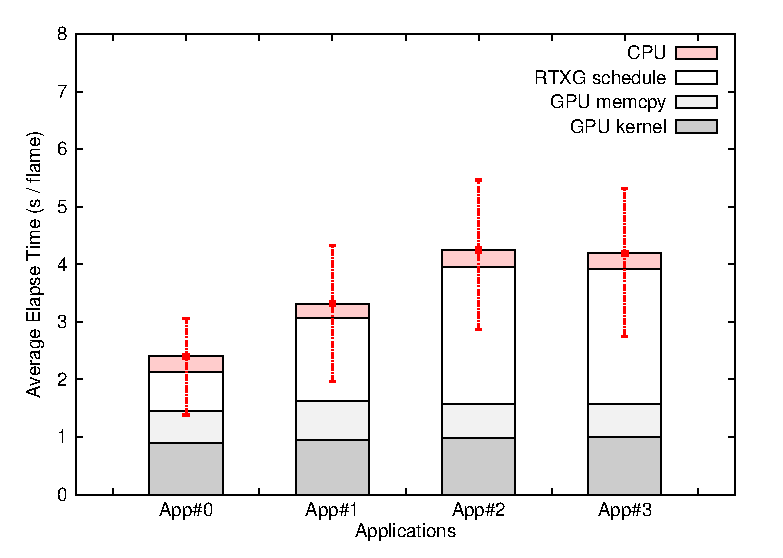
\includegraphics[width=62mm]{img/real_prio_band_withhighload_cpu}}
\label{fig:real-prio_band_cpu-hiload}
\end{center}
\end{minipage}
\caption{Execution time of the GPU-accelerated object detection program.}
\label{fig:elapse_time_all}
\end{figure*}

\SUBSECTION{Real-World Application}
We finally demonstrate the performance of Linux-RTXG on a real-world
application.
We tested with the GPU-accelerated object detection
program~\cite{hirabayashi:cpsna2013} based on the well-known DPM and HOG
algorithms.
We assume a monitoring system covering the four different directions to
East, West, South, and North.

We measure the execution time per frame in six different setups, as
shown in Figure~\ref{fig:elapse_time_all}, where no scheduling is
applied (a); fixed priorities are applied with GPU scheduling (b); GPU
resource reservation is further applied with the BAND scheduling policy
(c); and high CPU load is contending (d, e, f) with the $SCHED\_OTHER$
hackbench task.
The GPU tasks are allocated with $60\%$, $20\%$, $10\%$, and $10\%$ of
GPU reserves, respectively.

What we can obtain from this experiment is that if a high-CPU load task
exists, GPU tasks could be woefully affected in performance, since GPU
tasks can not acquire CPU time needed to execute the GPU API.
Linux-RTXG can provide both CPU scheduling and GPU scheduling with
resource reservation capabilities to solve this problem, as shown in
Figure~\ref{fig:elapse_time_all} (f).
As can be seen, the target programs are not affected by the high CPU
load task thanks to the $SCHED\_FIFO$ scheduling, while the GPU
execution can also be maintained at the desired frame rate thanks to the
GPU scheduling and resource reservation capabilities.
These results demonstrate that Linux-RTXG can supply prioritization and
QoS performance to real-world applications.

